% Copyright (C) 2005-2015 Airbus - EDF - IMACS - Phimeca
% Permission is granted to copy, distribute and/or modify this document
% under the terms of the GNU Free Documentation License, Version 1.2
% or any later version published by the Free Software Foundation;
% with no Invariant Sections, no Front-Cover Texts, and no Back-Cover
% Texts.  A copy of the license is included in the section entitled "GNU
% Free Documentation License".
\renewcommand{\filename}{docUC_InputWithData_LinearModel.tex}
\renewcommand{\filetitle}{UC : Estimation and validation of a linear model from two samples}

% \HeaderNNIILevel
% \HeaderIILevel
\HeaderIIILevel


\index{Regression Linear Model!Factory}
\index{Regression Linear Model!Cloud sample - Line graph}
\index{Regression Linear Model!Residual graph}
\index{Regression Linear Model!Adjusted Rsquared test@Adjusted $R^2$ test}
\index{Regression Linear Model!Rsquared@$R^2$ test}
\index{Regression Linear Model!Fisher test}
\index{Regression Linear Model!Residual test}

\index{Graph!Regression linear model}
\index{Graph!Residual Regression linear model}



The objective of this Use Case is to build a linear regression model between a the scalar variable $Y$ and the n-dimensional one $\vect{X} = (X_i)_{i \leq n}$, as follows :
\begin{align*}
  \tilde{Y} = a_0 + \sum_{i=1}^n a_i X_i + \varepsilon
\end{align*}
where $\varepsilon$ is the residual, supposed to follow the Normal(0.0, 1.0) distribution.\\
Each coefficient $a_i$ is evaluated from both samples {\itshape Ysample} and {\itshape Xsample} and is accompagnied by a confidence interval and a p-value (which tests if they are significantly different from 0.0).\\




Details on the linear regression model  may be found in the Reference Guide (\extref{ReferenceGuide}{see file Reference Guide - Step B -- Linear regression}{stepB}).\\



The linear model may be used to evaluate predictions on particular sample of the variable $X$ :  {\itshape particularXSample}.\\

The linear model may be validated :
\begin{itemize}
\item  graphically if {\itshape Xsample}  is of dimension 1, by drawing on the same graph the cloud ({\itshape Xsample, Ysample}) and the regression line, with the OpenTURNS method {\itshape DrawLinearModelVisualTest},
\item  numerically with the following OpenTURNS tests :
  \begin{itemize}
  \item {\itshape LinearModelRSquared} Test which tests the quality of the linear regression model. It evaluates the indicator $R^2$ (regression variance analysis) and compares it to a level,
  \item {\itshape LinearModelRAdjustedSquared} which  tests the quality of the linear regression model. It evaluates the indicator $R^2$ adjusted (regression variance analysis) and compares it to a level,
  \item {\itshape LinearModelFisher} Test which tests the nullity of the regression linear model coefficients (Fisher distribution used),
  \item {\itshape LinearModelResidualMean} Test which tests, under the hypothesis of a gaussian sample, if the mean of the residual is equal to zero. It is based on the Student test (equality of mean for two gaussian samples).
  \end{itemize}
\end{itemize}

The hypothesis on the residuals (centered gaussian distribution) may be validated :
\begin{itemize}
\item  graphically if {\itshape Xsample} is of dimension 1, by drawing the residual couples ($\varepsilon_i, \varepsilon_{i+1}$), where the residual $\varepsilon_i$ is evaluated on the samples  ({\itshape Xsample, Ysample}) : $\varepsilon_i = Ysample_i - \tilde{Y}_i$ with $\tilde{Y}_i = a_0 + a_1 Xsample_i$. The OpenTURNS method is {\itshape DrawLinearModelResidualtest} ,
\item  numerically with the {\itshape LinearModelResidualMean} Test which tests, under the hypothesis of a gaussian sample, if the mean of the residual is equal to zero. It is based on the Student test (equality of mean for two gaussian samples).
\end{itemize}

\longrequirements{
  \begin{description}
  \item[$\bullet$] a 1D-sample : {\itshape Ysample}
  \item[type:]  NumericalSample
  \item[$\bullet$] a nD-sample : {\itshape Xsample}
  \item[type:]  NumericalSample
  \item[$\bullet$] a nD-sample : {\itshape particularXSample}
  \item[type:]  NumericalSample
  \end{description}
}
                 {
                   \begin{description}
                   \item[$\bullet$] a linear regression model : {\itshape linearRegressionModel}
                   \item[type:]  LinearModel
                   \item[$\bullet$] the linear coefficients $(a_i)_{0 \leq i \leq n}$ : {\itshape coefValues}
                   \item[type:] scalarCollection
                   \item[$\bullet$] the confidence intervals of each coefficient $a_i$
                   \item[type:]  ConfidenceIntervalCollectionf
                   \item[$\bullet$] the p-values of each coefficient $a_i$
                   \item[type:]  ConfidenceIntervalCollection
                   \item[$\bullet$] the predicted value on a particular sample : {\itshape predictedSample}
                   \item[type:] NumericalSample
                   \item[$\bullet$] the sample of residual values: {\itshape residualSample}
                   \item[type:] NumericalSample
                   \item[$\bullet$] the graph superposing the samples cloud and the regression line (in case of dimension 1 for X) : {\itshape linearRegressionModel.png, linearRegressionModel.eps}
                   \item[type:]  files at format PNG or EPS or FIG
                   \item[$\bullet$] the graph of residual values : {\itshape residualGraph.png, residualGraph.eps}
                   \item[type:]  files at format PNG or EPS or FIG
                   \item[$\bullet$] LinearModelRAdjustedSquared test result : {\itshape resultLinearModelRAdjustedSquared}
                   \item[type:] TestResult
                   \item[$\bullet$] LinearModelRSquared test result : {\itshape resultLinearModelRSquared}
                   \item[type:] TestResult
                   \item[$\bullet$] LinearModelFisher test result : {\itshape resultLinearModelFisher}
                   \item[type:] TestResult
                   \item[$\bullet$] LinearModelResidualMean test result : {\itshape resultLinearModelResidualMean}
                   \item[type:] TestResult
                   \end{description}
                 }

                 \textspace\\
                 Python script for this UseCase :

                 \inputscript{script_docUC_InputWithData_LinearModel}

                 \textspace\\



                 The following figures draw the regression model superposed on the samples cloud ({\itshape Xsample, Ysample}) of size $10^3$ and the residuals graph in both cases :
                 \begin{itemize}
                 \item where the regression model seems validated : Figures  \ref{LMGood} and \ref{LMResidualGood},
                 \item where the regression model doesn't seem to be validated (relation of kind $Y = X^2$) : Figures  \ref{LMWrong} and \ref{LMResidualWrong}.
                 \item where the regression model doesn't seem to be validated (relation of kind $Y = sin(X)$) : Figures  \ref{LMWrong2} and \ref{LMResidualWrong2}.
                 \end{itemize}


                 \begin{figure}[H]
                   \begin{minipage}{8cm}
                     \begin{center}
                       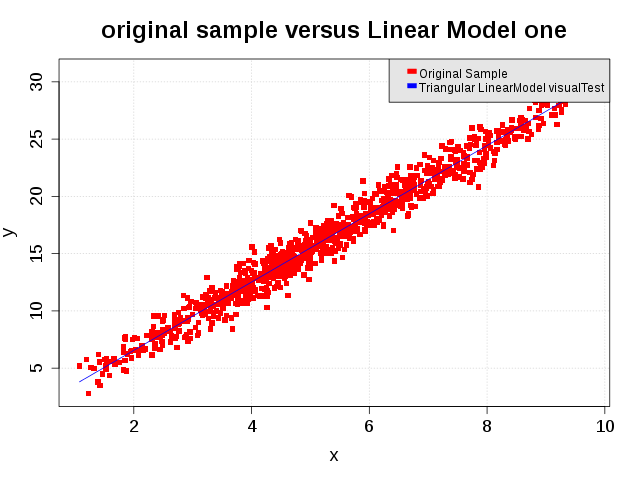
\includegraphics[width=8cm]{Figures/linearRegression_Graph.png}
                       \caption{Visual validation of the Linear Regression Model.}
                       \label{LMGood}
                     \end{center}
                   \end{minipage}
                   \hfill
                   \begin{minipage}{8cm}
                     \begin{center}
                       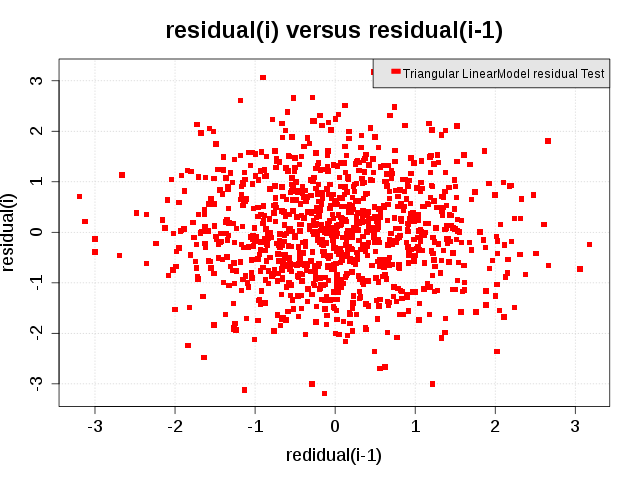
\includegraphics[width=8cm]{Figures/linearRegression_residualGraph.png}
                       \caption{Visual validation of the Linear Regression Model : residuals graph.}
                       \label{LMResidualGood}
                     \end{center}
                   \end{minipage}
                 \end{figure}



                 \begin{figure}[H]
                   \begin{minipage}{8cm}
                     \begin{center}
                       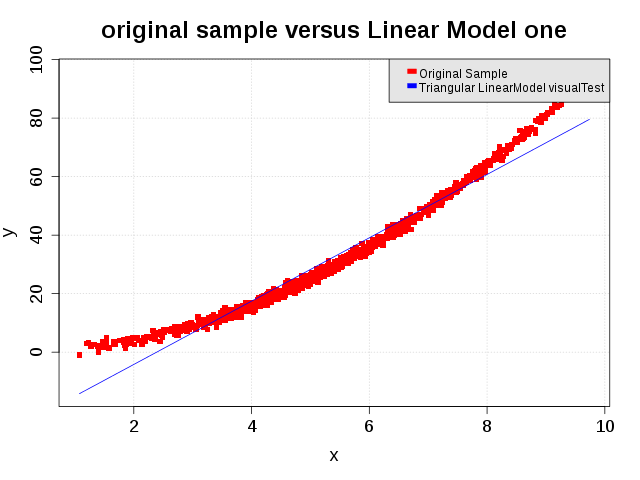
\includegraphics[width=8cm]{Figures/linearRegression_GraphWrong.png}
                       \caption{Visual invalidation of the Linear Regression Model.}
                       \label{LMWrong}
                     \end{center}
                   \end{minipage}
                   \hfill
                   \begin{minipage}{8cm}
                     \begin{center}
                       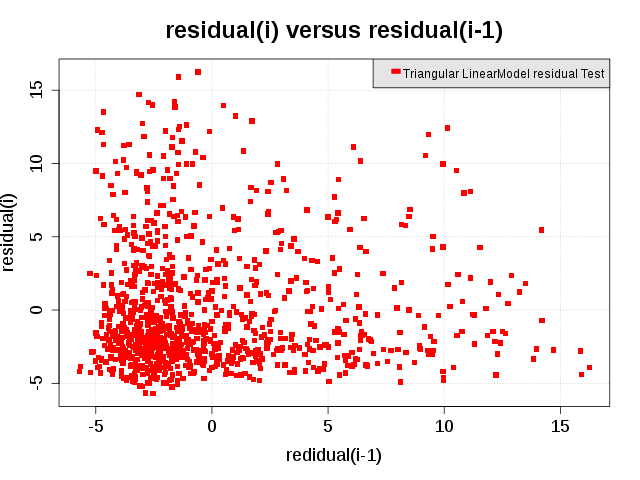
\includegraphics[width=8cm]{Figures/linearRegression_residualGraphWrong.png}
                       \caption{Visual invalidation of the Linear Regression Model : residuals graph.}
                       \label{LMResidualWrong}
                     \end{center}
                   \end{minipage}
                 \end{figure}


                 \begin{figure}[H]
                   \begin{minipage}{8cm}
                     \begin{center}
                       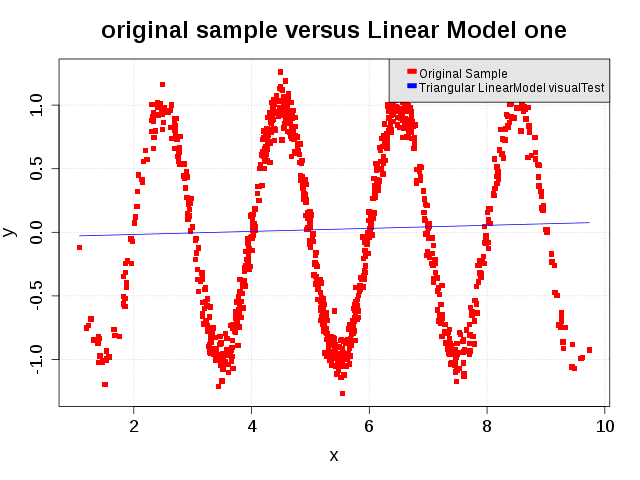
\includegraphics[width=8cm]{Figures/linearRegression_GraphWrong2.png}
                       \caption{Visual invalidation of the Linear Regression Model.}
                       \label{LMWrong2}
                     \end{center}
                   \end{minipage}
                   \hfill
                   \begin{minipage}{8cm}
                     \begin{center}
                       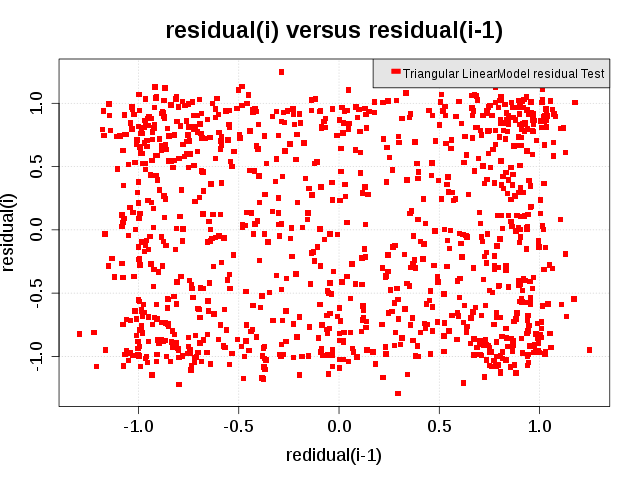
\includegraphics[width=8cm]{Figures/linearRegression_residualGraphWrong2.png}
                       \caption{Visual invalidation of the Linear Regression Model : residuals graph.}
                       \label{LMResidualWrong2}
                     \end{center}
                   \end{minipage}
                 \end{figure}
